\section{Auswertung}
\label{sec:Auswertung}

\subsection{Vorbereitungsaufgabe}
Als Vorbereitungsaufgabe für den Versuch wurden die Dopplerwinkel $\alpha$ zu den Prismenwinkeln $\theta = 15° , 30°$ und $60°$
mithilfe von \autoref{eqn:alpha} bestimmt.
Die Schallgeschwindigkeiten $c_L=\qty{1800}{\meter\per\second}$ und $c_P=\qty{2700}{\meter\per\second}$ werden hierbei der Versuchsanleitung
\cite{VUS3} entnommen.
Die Ergebnisse sind in \autoref{tab:vor} eingetragen.

\begin{table}
    \centering
    \caption{Prismenwinkel zu Dopplerwinkeln}
    \begin{tabular}{S[table-format=2.0] S[table-format=2.2]}
        \toprule
        {$\theta / \si{\degree}$} & {$\alpha  / \si{\degree}$}  \\
        \midrule
        15 & 80.06  \\
        30 & 70.53  \\
        60 & 54.74  \\
        \bottomrule
    \end{tabular}
    \label{tab:vor}
\end{table}

\subsection{Strömungsgeschwindigkeiten}
\label{sub:Strömungsgeschwindigkeiten}

Die Messung wird nach \autoref{sub:Strömungsgeschwindigkeiten_durch} durchgeführt und die Messwerte der Frequenzverschiebungen
zu den verschiedenen Pumpdrehzahlen in \autoref{tab:Mess1} eingetragen.
Außerdem wird mithilfe der nach $v$ umgestellten \autoref{eqn:Deltanu}
\begin{align}
  v= \frac{\Delta \nu \cdot c}{2 \nu_0 \cos{\alpha}} \label{eqn:v}
\end{align}
die Strömungsgeschwindigkeit des Mediums berechnet und der Tabelle hinzugefügt. 

\begin{table}
  \centering
  \caption{Gemessene Frequenzverschiebungen
          und die daraus errechneten Strömungsgeschwindigkeiten ($D_\text{groß} = \SI{16}{\milli\metre}$)}
  \label{tab:Mess1}
  \begin{tabular}{S[table-format=4.0]
                  S[table-format=3.0] S[table-format=1.2] 
                  S[table-format=3.0] S[table-format=1.3] 
                  S[table-format=4.0] S[table-format=1.3]}
      \toprule
      &
      \multicolumn{2}{c}{$\theta = \ang{15;;}$} &
      \multicolumn{2}{c}{$\theta = \ang{30;;}$} & 
      \multicolumn{2}{c}{$\theta = \ang{60;;}$} \\
      \cmidrule(lr){2-3} \cmidrule(lr){4-5} \cmidrule(lr){6-7}
      {$\text{rpm}$}&
      {$\symup{\Delta} \nu \mathbin{/} \si{\hertz}$} & {$v \mathbin{/} \si{\meter\per\second}$} & 
      {$\symup{\Delta} \nu \mathbin{/} \si{\hertz}$} & {$v \mathbin{/} \si{\meter\per\second}$} &
      {$\symup{\Delta} \nu \mathbin{/} \si{\hertz}$} & {$v \mathbin{/} \si{\meter\per\second}$} \\
      \midrule
      5000 & 208 & 0.54 & 377 & 0.51 & 670 & 0.52\\
      5250 & 275 & 0.71 & 428 & 0.58 & 753 & 0.59\\
      5500 & 309 & 0.81 & 500 & 0.68 & 840 & 0.65\\
      5750 & 339 & 0.88 & 563 & 0.76 & 938 & 0.73\\
      6000 & 375 & 0.98 & 612 & 0.83 & 1050 & 0.82\\
  \end{tabular}
\end{table}


  %Tabellen werte anpassen und andere 2 Tabellen noch erstellen!!!!!!!!!
  
  \begin{figure}[H]
    \centering
    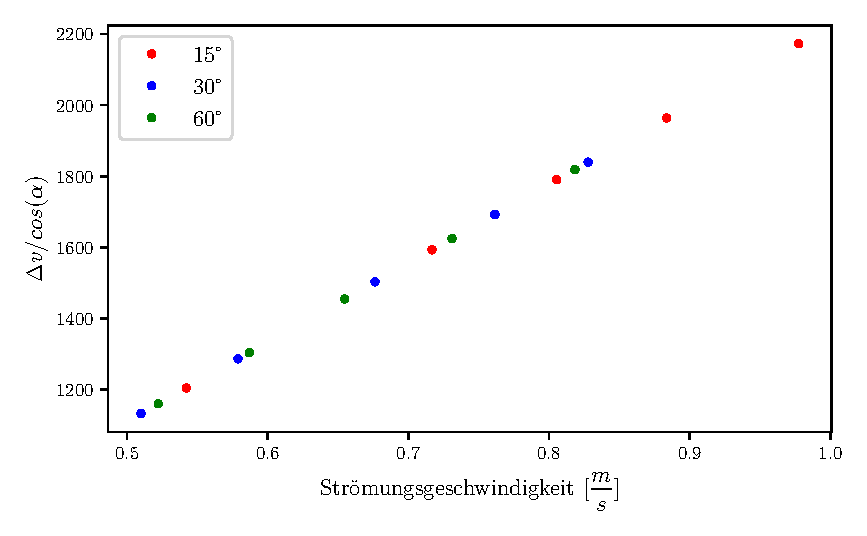
\includegraphics{build/plot1.pdf}
    \caption {Darstellung der Strömungsgeschwindigkeit gegenüber der Frequenzverschiebungen.}
    \label{fig:plot}
  \end{figure}

\subsection{Strömungsprofil}
\label{sub:Strömungsprofil}


\begin{table}
  \centering
  \caption{Prismenwinkel zu Dopplerwinkeln}
  \begin{tabular}{S[table-format=2.1] S[table-format=3.0] S[table-format=3.0] S[table-format=3.0]}
      \toprule
      {Messtiefe $d / \si{\micro\second}$}  & {Frequenzverschiebung $\symup{\Delta} \nu \mathbin{/} \si{\hertz}$} & {Intensität $I  / \si{\kilo\volt\squared\per\second}$} & {Geschwindigkeit $v  / \si{\meter\per\second}$} \\
      \midrule
      12,5  &  330 & 36  & \\
      13,0  &  373 & 48  & \\
      13,5  &  420 & 53  & \\
      14,0  &  455 & 61  & \\
      14,4  &  476 & 62  & \\
      15,0  &  461 & 70  & \\
      15,5  &  423 & 71  & \\
      16,0  &  368 & 77  & \\
      16,5  &  336 & 83  & \\
      17,0  &  373 & 75  & \\
      17,5  &  406 & 143 & \\
      18,0  &  410 & 344 & \\
      \bottomrule
  \end{tabular}
  \label{tab:vor}
\end{table}